\section{用GPU}
在Tensorflow中CPU,GPU用字符串表示
\begin{itemize}
\item "cpu:0":机器上的CPU
\item "gpu:0":机器上的GPU
\item "gpu:1":机器上的第二块GPU
\end{itemize}
 如果TensorFLow操作有GPU和CPU实现,GPU将被优先指定,例如matmul有CPU和GPU内核,在系统上 有cpu:0和gpu:0,gpu:0将优先运行matmul。
布置采集设备

找到你的操作和tensor上的设备,创建一个会话log\_device\_placement配置设置为True
\begin{python}
import tensorflow as tf
a = tf.reshape(tf.linspace(-1.,1.,12),(3,4))
b = tf.reshape(tf.sin(a),(4,3))
c = tf.matmul(a,b)
with tf.Session() as sess:
    print(sess.run(c))
\end{python}
输出参数:\newline
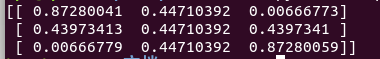
\includegraphics{./pic/chapter2/use_gpu1.png}\newline
\subsection{手工配置设备}
如果你想将你的操作运行在指定的设备中而不由tensorflow是自动为你选择,你可以用tf.device 创建一个设备,左右的操作将在同一个设备上指定。
\begin{python}
import tensorflow as tf
with tf.device('/cpu:0'):
    a = tf.constant([1.,2.,3.,4.,5.,6.],shape = (2,3),name = 'a')
    b = tf.reshape(a,shape=(3,2))
    c = tf.matmul(a,b)
    with tf.Session(config = tf.ConfigProto(log_device_placement=True)) as sess:
        print(sess.run(c))
\end{python}
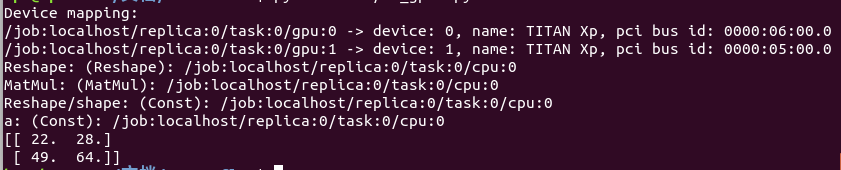
\includegraphics[scale=0.4]{use_gpu2.png}\newline
正如你看到的a,b被复制到cpu:0,因为设备没有明确指定,Tensorflow将选择操作和可用的设备(gpu:0)

\subsection{允许GPU的内存增长}

默认情况下Tensorflow将映射所有的CPUs的显存到进程上,用相对精确的GPU内存资源减少内存的碎片化会更高效。 通常有些程序希望分贝可用内存的一部分,或者增加内存的需要两。在会话中tensorflow提供了两个参数 控制它。 第一个参数是allow\_growth选项,根据运行情况分配GPU内存:它开始分配很少的内存,当Session开始运行 需要更多GPU内存是,我们同感Tensorflow程序扩展GPU的内存区域。注意我们不释放内存,因此这可能导致更多的内存碎片。为了开启这个选项,可以通过下面的设置
\begin{python}
config = tf.ConfigProto()
config.gpu_option.allow_growth = True
sess = tf.Session(config=config,...)
\end{python}
第二种方法是per\_process\_gpu\_memory\_fraction选项,决定GPU总体内存中多少应给被分配,例如你可以告诉 Tensorflow分配40\%的GPU总体内存。
\begin{python}
config = tf.ConfigProto()
config.gpu_option.per_process_gpu_memory_fraction = 0.4
sess = tf.Session(config = config)
\end{python}
如果你想限制Tensorflow程序的GPU使用量,这个参数是很有用的。

在多GPU系统是使用GPU

如果你的系统上有超过一个GPU,你的GPU的抵消的ID将被默认选中,如果你想运行在不同的GPU上,你需要指定 你想要执行运算的GPU
\begin{python}
import tensorflow as tf
with tf.device('/gpu2:0'):
    a = tf.constant([1.,2.,3.,4.,5.,6.],shape = (2,3),name = 'a')
    b = tf.reshape(a,shape=(3,2))
    c = tf.matmul(a,b)
    with tf.Session(config = tf.ConfigProto(log_device_placement=True)) as sess:
        print(sess.run(c))
\end{python}
如果你指定的设备不存在,你将个到一个InvalidArgumentError:\newline
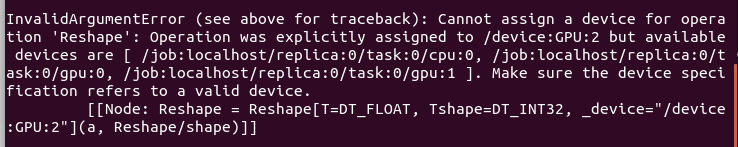
\includegraphics[scale=0.4]{use_gpu3.png}\newline
如果你想Tensorflow在万一指定的设备不存在时自动选择一个存在的设备,你可以在创建会话时配置中设置allow\_soft\_placement 为True
\begin{python}
with tf.device('/gpu:2'):
  a = tf.constant([1.,2.,3.,4.,5.,6.],shape= [3,2],name = 'a')
  b = tf.constant([1.,2.,3.,4.,5.,6.],shape= [2,3],name = 'b')
  c = tf.matmul(a,b)
with tf.Session(config = tf.ConfigProto(allow_soft_placement=True,log_device_placement=True)) as sess:
    print(sess.run(c))
\end{python}
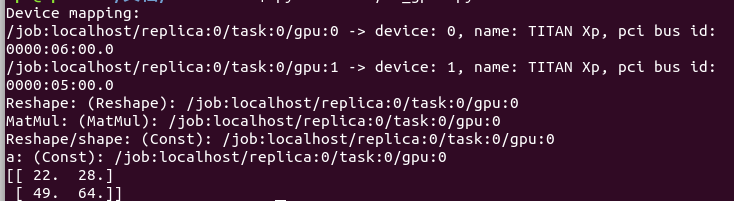
\includegraphics[scale=0.4]{use_gpu4.png}\newline
用多GPU

如果你想在多张GPU上运行Tensorflow,你可以在multi-tower fashion上构造你的模型,每个tower 被指定到不同的GPU上。例如:
\begin{python}
c = []
for d in ['/gpu:0', '/gpu:1']:
    with tf.device(d):
        a = tf.constant([1.0, 2.0, 3.0, 4.0, 5.0, 6.0], shape=[2, 3])
        b = tf.constant([1.0, 2.0, 3.0, 4.0, 5.0, 6.0], shape=[3, 2])
        c.append(tf.matmul(a, b))
    with tf.device('/cpu:0'):
        sum = tf.add_n(c)
   # Creates a session with log_device_placement set to True.
sess = tf.Session(config=tf.ConfigProto(allow_soft_placement=True,log_device_placement=True))
  # Runs the op.
print(sess.run(sum))
sess.close()
\end{python}
\section{如何利用Inception的最后一层重新训练新的分类}
现代的认知模型可能有上百万个参数可能需要花几周训练,Transfer学习是通过完整的像ImageNet一样的模型通过已经存在的权重简化数周工作分类的技术。在这个例子中我们将创新训练最终层不修改其它层。详细信息你可以查看\href{http://arxiv.org/pdf/1310.1531v1.pdf}{这篇论文}.

尽管不完整的训练,但是对于一些应用却惊人的高效,可以在笔记本上训练30分钟,不要求GPU。这个导航将显示给你如何在自己的图像运行示例脚本解释一些控制训练需要的脚本。
\subsection{训练花}
\begin{center}
\begin{figure}
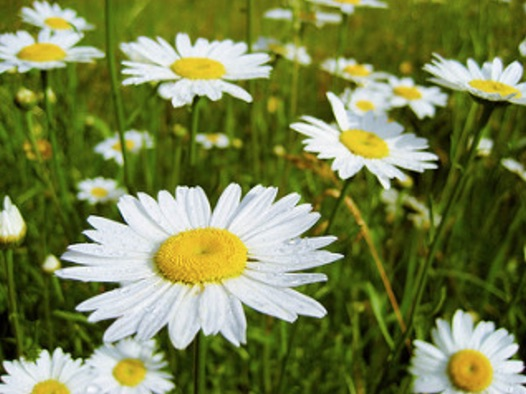
\includegraphics[scale=0.5]{daisies.jpg}
\end{figure}
\end{center}
在开始训练前你需要设置图像教网络你想认识的新的类别。接下来的张杰解释如何准备你的图像,但是我们创建一个授权的归档的花的文件使得训练更轻松。为了得到花的图像,运行下面的代码:
\begin{lstlisting}[language={[ANSI]C}]
cd ~
curl -O http://download.tensorflow.org/example_images/flower_photos.tgz
tar xzf flower_photos.tgz
\end{lstlisting}
当你有图像后,你从你的TensorFlow源文件目录构建重新训练器
\begin{lstlisting}[language={[ANSI]C}]
bazel build --config opt tensorflow/examples/image_retraining:retrain
\end{lstlisting}
可以通过下面运行:
\begin{lstlisting}{language=[ANSI]C}
bazel build tensorflow/examples/image_retraining:retrain
\end{lstlisting}
如果你有一个机器支持AVX设备集(最近几年的常用的x86 CPUs)你可以通过架构提高building运行速度
\begin{lstlisting}{language=[ANSI]C}
bazel build --config opt tensorflow/examples/image_retraining:retrain
\end{lstlisting}
训练器可以是这样:
\begin{lstlisting}{language=[ANSI]C}
bazel-bin/tensorflow/examples/image_retraining/retrain --image_dir ~/flower_photos
\end{lstlisting}
这个脚本载入先前incption v3模型,删除顶层,在新的flower photos训练新的模型。在原始ImageNet类中没有一种花完整网络被完整的训练过了,transfer学习是低层已经被训练好
区别不修改任何不同对象。
\subsection{瓶颈}
训练花费30分钟甚至更长时间取决于你的机器的速度。第一个时期分析所有磁盘上的图像和计算他们的瓶颈,瓶颈是一个信息对术语
我们经常在最后一层前一层,倒数第二层已经训练区别输出要求分类的值,这意味着这必须是有意义的,因此对于分类器它必须包含足够的信息在一些小的值得集合中做选择,这意味着我们的最终层训练可以在新的类中工作证明在ImageNet中1000类对于区别新的对象是有用的。
因为每个图像在训练和计算花费时间瓶颈时被多次使用,他的速度达到缓存起的瓶颈因此不能被重复计算。默认他们存储在/tmp/bottleneck陌路,如果你仍然会脚本他们将被重用,因此你不是必须再次等待这部分。
\subsection{训练}
当瓶颈计算完成时,实际顶层训练开始。你讲看到输出,显示精度,可用精度,交叉熵。训练精度显示在当前训练批中多少被分类正确,验证训练精度从图像数据集随机选中精度的值,不同之处在于训练精度基于网络已经学习到的参数,在训练中可能过拟合到为噪声。验证精确度用不在训练集中的数据性能测量精确度,如果训练精确度很高,测试精确度很低说明网络过拟合训练图像存储的部分参数没有用。交叉熵损失函数查看学习进程处理的增么样,训练对象使得损失尽可能小,因此你可以分辨出如果学习起作用,忽略损失噪声损失保持下降的趋势。默认脚本运行4000步,每一步从训练集中随机选择10张图像找到缓冲器的瓶颈,输入数据仅最终层预测。预测然后比较实际label和真实值差距反向传递误差。当你继续的时候你应该看到精确度的提高。你应该能看到精确度在90\%到95\%之间,通过提取值将随机的一次次训练,这个数完全训练好模型后基于在给定测试集中正确标签的百分比。
\subsection{用TensorBoard可视化}
包含TensorBaord总结的脚本吗很容易理解,调试,优化。例如,你可以可视化图和统计,例如在训练中权重和精度变化:
\begin{lstlisting}{language=[ANSI]C}
tensorbaord --logdir /tmp/retrain_logs
\end{lstlisting}
TensorBoard运行后导航到localhost:6006查看TensorBoard,脚本将默认采集TensorBoard总结到/tmp/retain\_logs,你可以通过summaries\_dir标志指定采集目录。
\subsection{用重新训练的模型}
脚本将用训练好的最后一层写出你的一个Inception v3版本到/tmp/output\_graph,text文件在/tmp/output\_labels.txt包含标签,两个格式见
\href{https://www.tensorflow.org/tutorials/image_recognition}{C++ and Python image classification examples},因此你可以立即开始新的模型。你去带最顶层,你将需要在脚本中指定新的名字,例如你用label\_image,用--outout\_layer=final\_result.
你可以用下面的代码重新训练图:
\begin{lstlisting}{language=[ANSI]C}
bazel build tensorflow/examples/image\_retraining:label\_image && \
bazel-bin/tensorflow/examples/image_retraining/label_image \
--graph=/tmp/output_graph.pb --labels=/tmp/output\_labels.txt \
--image=$Home/flower_photos/daisy/21625746_cc379eea_m.jpg
\end{lstlisting}
你应该看到花的标签的列表在大说书情况下daisy在顶层(尽管重新训练的模型被可能会一点不同),你可以用在你的图片上--image参数
用c++代码作为模板整合你自己的应用。
如果你想在自己的Python程序中用你训练好的模型,上面的\href{https://www.github.com/tensorflow/tensorflow/blob/r1.3/tensorflow/examples/image_retraining/label_image.py}{label\_image script}
如果你发现默认的Inception v3模型对你的应用太大或者太慢,看看\href{https://www.tensorflow.org/tutorials/image_retraining#other_model_architectures}{Other Model Architechtures section}
\subsection{在你自己的分类上训练}
如果你已经成功的让脚本在花的例子上工作,你可以教他认识其他你想它认识的东西。理论上你需要设置一个子文件夹,命名分类,每个文件夹包含分类的图像。如果你传递子文件夹的根文件夹作为参数给--image\_dir,脚本像上面训练花一样训练。
\begin{center}
\begin{figure}
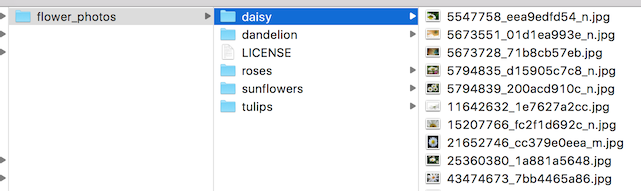
\includegraphics[scale=0.5]{folder_structure.png}
\end{figure}
\end{center}
实际上它会花一点时间得到你想要的精度,下面是一些常见的问题。
\subsection{创建一个训练图像集合}
首先我们需要查看收集到的图像,常见的问题是训练过程中数据的输入。

为了训练能起作用,每个你想要识别的图像你必须至少手机100张图片,你收集到的图片越多,训练的精确度可能越好。例如你拍摄一些蓝色的房间,另一些是绿色的房间模型的预测最终基于背景颜色,没有对象特征被考虑。为了避免这种情况,拍摄不同颜色的,没有一些实际能看到的的特征。如果你想了解更多这类问题你需要读\href{http://www.jefftk.com/p/detecting-tanks}{tank recognition}
如果你想考虑你用的分类。分隔大的数据集发现一些不同的物理形式为小的可以通过视觉区分的数据集,例如你可以用'vehicle'可以用来替代
'car','motobike'和'truck',考虑你有一个开放的世界还是封闭的世界将是很有价值的,在封闭的世界你唯一需要考虑的是识别已有的对象,例如一个植物识别的app你应该知道用户可能拍摄的花的图片,英雌你必须决定花的种类,相比之下一个巡逻机器人可能通过摄像头看到不同的事物。在这种情况下你想要分类器报告是否确认他看到的,这可能很难,但是你经常收集一些典型的和主体对象不相关的背景图像,,你可能会让它增加一些图片文件夹中未知的分类。
检查确保你的图像被正确的标记也是很重要的。经常用生成的标签对于你的目的来说是不可靠的,例如你用\#daisy命名一个叫Daisy的人。如果你想你的图像如果你了解你的图像,扫除任何错误将可能导致最后精确度提高。
\subsection{训练步骤}
如果你为你的图片感到高兴,你可以通过修改学习进程中的细节提升你的结果。最简单的方法是用--how\_many\_training\_steps。默认是4000.但是如果你增加到8000,他的训练时间将增加到两倍。精确度提高的比率显示你训练的越长一些点将停止,但是你可以试验什么时候达到你的模型的限制。
\subsection{扭曲}
随机通过变形,剪裁,变化输入图像的亮度是一个提高结果的常用方法,这样扩展了训练数据的大小,帮助网络学习
真是生活分类器所有的扭曲,在脚本中使用扭曲最大的缺点是缓冲瓶颈不再有用,因此输入图像将不能重用。这意味着训练京城可能花费更多时间,因此我推荐当着作为一个调节方法调节你的模型到合理。
你可以传递--random\_corp,--random\_scale和--random\_brightness给脚本扭曲图片。百分比值用来控制图片上扭曲用多少部分。,合理的值时5或者10.--flip\_left\_right将在水平方向随机的镜像图像的一半,有助有你的应用能理解翻转的图像。例如如果你想识别字母这将不是一个好的办法,因为翻转它们会毁掉原来的含义。
\subsection{超参数}
你可以调整一些参数查看是否对你的结果有帮助,--learning\_rate控制最终层训练更新的幅度。直观理解,如果这个值变小训练时间将边长,但是他可能对精度有帮助,你需要小心试验得到查看什么对于你的case生效了。--train\_batch\_size控制每一训练步多少图像被检查,因为学习率应用到每批上,如果你有更大的批得到相同的效果你将需要减小它。
\subsection{训练,验证,测试集}
当你为你的脚本指定图像文件夹时,文件夹被分成不同的数据集。最大的数据及是训练集,训练集包含用于训练网络的数据,用于更新权重。你也许很想知道为什么我们不用所有的图像训练?一个道德潜在的问题是当我们做机器学习算法时我们的模型会记住接近正确答案的不相关信息,你可以想想你的图像可能记住了一些照片的背景,通过标签匹配对象,它在训练时所有的图像可能产生一个好的结果,但是不能再新的图像产生好的结果因为他不能泛化对象的特征,仅仅在训练图像的时候记住了一些不重要的特征。
这个问题被称为过拟合,为了避免过拟合我们保持我们的一些数据不再训练进程中,因此模型不能记住他们,我们用这些图像作为检察确保过拟合没有发生,当我们在看模型在这些数据上有一个好的精度说明过拟合没有发生,通常80\%的数据被用来作为训练集10\%的数据集用来验证最后10\%的数据用做测试集预测分类器在真实世界的性能,通过--testing\_percentage和--validation\_percentage标志用来控制比例。通常你应该能留下一些值作为默认,不应该找到任何好处训练调整他们。
注意这个脚本用图象的文件名区分训练集,验证集,测试集中的图像(不是一个随机的函数),这样保证运行时图片不会再训练集和测试集之间移动,因为当用于训练模型的图像被验证集中的图像取代时可能会出现一些问题。
你也需注意到了在迭代过程中验证正确度的波动。多数波动是验证集的子集的随机性引起的,选择的验证集用来验证精确度。波动能能被最大层度减少,花费的训练时间增长,通过选择--validation\_batch\_size=-1用整个验证集计算精度。
当训练结束后你将能检查测试集中错误分类图像,这可以通过增加--print\_misclassified\_test\_images标记,这对于找到那些什么类型的图片让模型困惑(很难区别的)是很有帮助的例如你也许发现了一些种类一些常见的图像角度是特别难是别的,这样是鼓励你增加更多类型的分类训练子类,检查催哦五分类图片也指出输入数据中的错误,向错误标签,其质量魔术的照片。然而,你应该避免测试集固定点单个误差,因为他们仅仅反映在训练集中更多的问题。
\subsection{更对模型架构}
这个脚本默认用Inception v3模型架构作为预先训练脚本。这是一个好的开始的地方,因为它提供了高精度的训练结果,但是如果你想部署你的模型到手机设备或者其他的资源限制的环境你也许想要这种精确度换区更小的文件尺寸和更快的速度。
为了帮助这个\href{https://github.com/tensorflow/tensorflow/blob/master/tensorflow/examples/image_retraining/retrain.py}{retrain}
在\href{https://research.googleblog.com/2017/06/mobilenets-open-source-models-for.html}{移动架构}上支持30个不同的变量。
这里有一些比Inception v3更小精度的,但是可以得到更小的文件大小(下载小于兆字节)运行快乐几倍。为了训练这个模型,传递--architecture标志,例如:
\begin{lstlisting}{language={ANSI}C}
python tensorflow/examples/image_retraining/retrain.py \
    --image_dir ~/flower_photos -- architecture mobilenet_0.25_128_quantized
\end{lstlisting}
这将在/temp/创建一个941KB模型文件output\_graphi.pb.Mobilenet的25\%的参数,占据$128\times128$大小的输入图像,权重在磁盘中量化为8位,你可以选择'1.0','0.75','0.50','0.25'控制权重参数的数量,因此文件尺寸(和一些扩展速度),'224','192','160'或者'128'对于输入图像的尺寸,更小的尺寸更快的速度,选项'\_quantized'预示着是否文件应该包含8位或者32位浮点权重。速度和大小好处带来的是精确度的损失,但是对于一些用途来说是不重要的,他可以通过训练数据提高、例如用扭曲在花数据集允许你得到得到80\%的精度,甚至0.25/128、quantized图。
如果你在你的程序或者label\_image中用Mobilenet模型,你讲需要一个输入一个指定大小的图像转换一个浮点让位到'input' tensor,典型的24位乳香范围[0,255]你必须用(image-128.)/128转化它到[-1,1]范围。
\section{TF layer向导:建立一个卷积神经网络}
TensorFlow\href{https://www.tensorflow.org/api_docs/python/tf/layers}{layers module}是一个用于轻松建立神经网络的高级API,它提供了一个方法促进创建dense(全连接)层和卷积层,增加激活函数,应用dropout规则。在这个导航中,你讲学习如何用layers建立一个卷积神经网络模型识别手写体数据集。
\textbf{手写体数据集包含0-9,60000个训练样本10000个测试样本,图像格式为}$28\times28$
\subsection{开始}
创建文件cnn\_mnist.py,在手写体程序中添加如下代码:
\begin{python}
from __future__ import absolute_import
from __future__ import division
from __future__ import print_function

# Imports
import numpy as np
import tensorflow as tf

tf.logging.set_verbosity(tf.logging.INFO)

# Our application logic will be added here

if __name__ == "__main__":
  tf.app.run()
\end{python}
正如你看到的,你将增加,构造,训练,评估卷积神经网络,最终代码可以点击\href{https://www.github.com/tensorflow/tensorflow/blob/r1.3/tensorflow/examples/tutorials/layers/cnn_mnist.py}{这里}
\subsection{介绍卷积神经网络}
卷积神经网络是当前最先进的用于图像分类任务的模型架构。CNNs应用一些滤波器从原始的图像像素中提取高级特征,这个模型可能被用在分类。CNN包含三个组件:
\begin{itemize}
  \item \textbf{卷积层} 应用指定数量的卷积滤波器在图像上。对于每一个子区域,layer执行一系列数学操作生成一个单个值在输出feature map,卷积层然后应用relu激活函数输出非线性。
  \item \textbf{池化层} 下采样卷积层的图像数据,减小feature map的维度从而减小处理时间。常用池化算法是最大池化(提取feature map子区域)保留最大值,丢掉其它值。
  \item \textbf{Dense layers(全连接层)}在通过卷积层和下采样层特征提取执行分类。在全连接层,每一个节点连接到前面的节点。
\end{itemize}
通常CNN有一个卷积模块组成,每个层有卷积模块和池化模块组成。最新的卷积模块有一个或者更多的全连接层链接执行分类。最终CNN的全连接层包含每个目标类的一个单个节点(所有模型可能预测的类),用sofymax函数生成一个0-1的值(所有值的和维1)。我们可以解释给定图像和目标的相似情况。
\subsection{建立CNN MNIST分类器}
用CNN架构建立模型分类MNIST数据集。
\begin{enumerate}
  \item 卷积层1:应用$5\times5$卷积核(提取$5\times5$像素的区域),用relu激活函数。
  \item 池化层1:执行最大池化$2\times2$stride=2(指定的池化区域不重叠)
  \item 卷积层2:应用64个$5\times5$的卷积核,激活函数为relu。
  \item 池化层2:再次执行最大池化操作(卷积核$2\times2$)strider=2。
  \item Dense1:1024个神经元,dropout=0.4。
  \item Dense2:10个神经元0-9。
\end{enumerate}
打开cnn\_mnist.py增加下面的符合TensorFlow's Estimator api接口的cnn\_model\_fn函数。cnn\_mnist.py接受mnist特征数据,标签,\href{https://www.tensorflow.org/api_docs/python/tf/estimator/ModeKeys}{模型}作为参数,配置CNN,返回预测,损失,训练操作。
\begin{python}

\end{python}
下面的章节函数深入tf.layers代码创建每一层,如何计算loss,配置训练操作,生成预测。auguries你已经体验过CNN设TensorFlow Estimators,你可以跳到\href{https://www.tensorflow.org/tutorials/layers#training-and-evaluating-the-cnn-mnist-classifier}{Training and Evaluating the CNN MNIST Classifier}
\subsection{输入层}
 这个方法为二维图像数据创建见卷积和池化,输入tensor的形状为[batch\_size,image\_width,image\_height,channels]
\begin{itemize}
\item batch\_size:在训练过程执行提图下降的样本数据的子集大小。
\item image\_width:样本图像的宽。
\item image\_height:样本图像的高。
\item channels:样本图像的颜色通道,对于彩色图想,通道为3,对于单色图像通道为1.
\end{itemize}
在这里,我们的MNIST数据集由$28\times28$像素的单色照片组成,因此输入层的形状为[batch\_size,28,28,1],转变我们的feature map到这个形状,你可以执行操作:
\begin{python}
input_layer = tf.reshape(features["x"],[-1,28,28,1])
\end{python}
这里的-1表示输入的features["x"]的值的batch size应该被动态计算,保持所有的其它维度为常数。这允许我们将batch\_size作为一个可以调节的超参数。例如,如果我们输入样本到我们的batchs是5的模型,features["x"]将包含3920($5\times28\times28$)值(每一个值代表一个像素点),input\_layer形状将为[5,28,28,1],类似的如果我们样本的batchs是1000,features["x"]将包含78400个值,input\_layer形状将为[100,28,28,1]。
\subsection{第一层卷积层}
在我们的卷积层我想用32个$5\times5$的卷积核到输入层,用ReLU激活函数,我们一可用conv2d()方法创建这个层:
\begin{python}
conv1 = tf.layers.conv2d(
    inputs=input_layers,
    filters=32,
    kernel_size=[5,5],
    padding="same",
    activation=tf.nn.relu
)
\end{python}
\begin{displayquote}
inputs参数指定我们的输入tensor(形状为[batch\_size,image\_width,image\_height,channels]),这里,我们链接我们的第一个吉安基层到输入层,形状为[batch\_size,28,28,1]
注意:如果传递参数data\_format=channels\_first,conv2d()接受[channels,batch\_size,image\_width,image\_height]形状的数据。
\end{displayquote}
filter参数制定卷积核的个数,这里卷积核为32个。kenel\_size制定卷积核的维度为[width,height](这里[5,5])
padding参数制定两个值:valid(默认),和same。制定输出tensor应该有和输入特纳是哦然相同的形状,我们设置padding=same,说明TensorFLow增加0值到输出tensor的边缘波啊池宽度和高度为28(没有padding$5\times5$卷积$28\times28$将生成$24\times24tensor$,在$28\times28$用$5\times5$提取出$24\times24$个位置)。
activation参数指定应用到输出的激活函数,这里我们只顶tf.nn.relu。
conv2d()的输出形状为[batch\_size,28,28,32]:和输入有相同的宽度和高度,但是有32个通道保持每个卷积核的输出。
\subsection{池化层1}
链接我们创建的卷积层和池化层,我们在layers中用max\_pooling2d()方法构造执行最大池化,卷积核filter大小为$2\times2$,stride为2。
\begin{python}
pool1 = tf.layers.max_pooling2d(inputs=conv1, pool_size=[2, 2], strides=2)
\end{python}
再次,inputs制定输入tensor,形状为[batch\_size,image\_width,image\_height,channels],这里我们的输入tensor是第一层卷积层的输出conv1,形状为[batch\_size,28,28,32]

pool\_size指定最大池化filter的大小作为[width,height](这里是[2,2])如果两个维度相等你可以指定pool\_siz=2。
strides参数制定stride的大小,这里我们设置strdes为2,表示通过filter提取子区域的时候宽度和高度都是2像素。如果你想设置不同的width和height,你可以制定一个元祖或者列表。

我们的输出特纳是哦然和max\_pooling2d(pool1,形状为[batch\_size,14,14,32])相乘:$2\times2$减少宽度和高度到50\%。
\subsection{二层卷积和池化}
我们用conv2d()和max\_pooling2d()链接卷积和池化。对于卷积层2,我们配置64个$5\times5$的卷积核,激活函数为ReLU,池化层2,我们用和池化层一眼个间隔:
\begin{python}
conv2 = tf.layers.conv2d(
    inputs=pool1,
    filters=64,
    kernel_size=[5, 5],
    padding="same",
    activation=tf.nn.relu)

pool2 = tf.layers.max_pooling2d(inputs=conv2, pool_size=[2, 2], strides=2)
\end{python}
卷积层用pool1作为输入,生成tensor conv2。conv2形状为[atch\_size,14,14,64],和pool1的宽和高相等,64个通道因为64个卷积核。

池化层2那conv2作为输入,生成pool2作为输出,pool2形状[batch\_size,7,7,64](减少conv2 50\%的宽度和高度)
\subsection{Dense layer}
我们添加dense层(1024个神经元和ReLU激活函数)到CNN生成卷积/池化层提取的特征分类,我们将flatten我么呢feature map(pool2)到形状[batch\_size,features],因此我们的tensor有两维,上面的形状变成了[batch\_size,$7\times7\time64$]:
\begin{python}
pool2_flat = tf.reshape(pool2, [-1, 7 * 7 * 64])
\end{python}
现在哦我们用dense方法链接我们的dense:
\begin{python}
dense = tf.layers.dense(inputs=pool2_flat, units=1024, activation=tf.nn.relu)
\end{python}
inputs参数制定输入tensor:我们的flattened的feature map pool2\_flat。units参数指定dense层的神经元的数量。activation参数获取激活函数,这里我们依然是用tf.nn.relu。
为了改进我们的模型,我们也应用dropout方法正则化dense层。
\begin{python}
dropout = tf.layers.dropout(
    inputs=dense, rate=0.4, training=mode == tf.estimator.ModeKeys.TRAIN)
\end{python}
inputs参数和上面一样,rate参数制定dropout比率,这里用0.4表示40\%的元素将在训练中被随机丢弃。training参数得到一个bool行值制定是否模型在训练模式下运行,dropout仅仅在training为True时执行。这里我们检查是否mode传递给我们cnn\_model\_fn的模型函数是TRAIN模式。输出形状为[batch\_size,1024]
\subsection{Logits Layers}
在我们神经网络的最后一层是logits层,然会预测的原始值。我们用10个神经元创建一个dense layers,激活函数哦认为线性激活函数。
\begin{python}
logits = tf.layers.dense(inputs=dropout, units=10)
\end{python}
我们最终输出CNN的tensor,logits形状为[batch\_size,10]。
\subsection{常见的预测}
logits层返回我们预测的原始值(形状[batch\_size,10])。让我们转化这些原始值到我们的模型函数能返回的两种个不同的格式。
\begin{itemize}
\item predicted class:数字0-9。
\item probabilities:对于每个可能的目标类的概率。
\end{itemize}
对于更定的例子,我们的预测类是在相关行logts列有最大的值。我们可以用该tf.argmax函数找到这个元素的索引。
\begin{python}
tf.argmax(input=logits, axis=1)
\end{python}
input参数制定需要提取最大值的tensor,axis参数制定输入tensor沿着哪个轴寻找最大值。这里我们写着1轴寻找最大值。
我们可以用softmax生成概率。
\begin{python}
tf.nn.softmax(logits, name="softmax_tensor")
\end{python}
我们融合我们的预测到一个字典中,返回一个EstimatorSpec对象。
\begin{python}
predictions = {
    "classes": tf.argmax(input=logits, axis=1),
    "probabilities": tf.nn.softmax(logits, name="softmax_tensor")
}
if mode == tf.estimator.ModeKeys.PREDICT:
  return tf.estimator.EstimatorSpec(mode=mode, predictions=predictions)
\end{python}
\subsection{计算Loss}
对于训练和评估阶段,我们需要定义损失函数衡量我们的模型的预测如何接近目标类。对于想MNIST的多个分类问题,\href{https://en.wikipedia.org/wiki/Cross_entropy}{cross entropy}是典型的被用做损失度量。下面的代码计算交叉熵返回TRAIN或者EVAL模式:
\begin{python}
onehot_labels = tf.one_hot(indices=tf.cast(labels, tf.int32), depth=10)
loss = tf.losses.softmax_cross_entropy(
    onehot_labels=onehot_labels, logits=logits)
\end{python}
我们的labels tensor包含一个预测列表,像[1,9,\ldots],为了计算交叉熵,你需要转换labels为相关的\href{https://www.quora.com/What-is-one-hot-encoding-and-when-is-it-used-in-data-science}{one-hot encoding}
\begin{python}
[[0, 1, 0, 0, 0, 0, 0, 0, 0, 0],
 [0, 0, 0, 0, 0, 0, 0, 0, 0, 1],
 ...]
\end{python}
womenyoingtf.one\_hot函数执行转换。tf.one\_hot()有两个参数:
\begin{itemize}
\item one-hot tensor有值的位置,如上面1,表示位置索引为1的地方有1
\item depth:one-hot tensor的深度,目标类的数量,这里depth为10,
\end{itemize}
下面的代码为我们的labels创建一个one-hot tensor,onehot\_labels:
\begin{python}
onehot_labels = tf.one_hot(indices=tf.cast(labels, tf.int32), depth=10)
\end{python}
因为labels包含值从0-9,indices是我们的labels tensor,值变为证书。depth是10因为我们有10个可能的目标类。
下一步我们计算onehot\_labels的交叉熵和我们的logits层的softmax预测。tf.losses.softmax\_cross\_entropy()得到onehot\_labels和logits作为参数。在logits上执行softmax激活函数,返回损失的标量tensor:
\begin{python}
loss = tf.losses.softmax_cross_entropy(
    onehot_labels=onehot_labels, logits=logits)
\end{python}
\subsection{配置训练操作}
在先前的操作中我们为我们的CNN定义了损失作为logits层和layers的softmax cross-entropy。让我们配置我们的模型在训练落成中优化loss。我们将用0.001学习率和\href{https://en.wikipedia.org/wiki/Stochastic_gradient_descent}{SGD}作为优化算法\begin{python}
if mode == tf.estimator.ModeKeys.TRAIN:
  optimizer = tf.train.GradientDescentOptimizer(learning_rate=0.001)
  train_op = optimizer.minimize(
      loss=loss,
      global_step=tf.train.get_global_step())
  return tf.estimator.EstimatorSpec(mode=mode, loss=loss, train_op=train_op)

\end{python}
\subsection{增加评估度量}
为了增加度量到我们的模型,我们在EVAL定义了eval\_metric\_ops字典:
\begin{python}
eval_metric_ops = {
    "accuracy": tf.metrics.accuracy(
        labels=labels, predictions=predictions["classes"])}
return tf.estimator.EstimatorSpec(
    mode=mode, loss=loss, eval_metric_ops=eval_metric_ops)
\end{python}
\section{训练评估CNN MNIST分类器}
我们已经构建了MNIST CNN模型函数,现在我们准备训练评估它。
\subsection{载入训练和测试数据}
增加main()函数到cnn\_mnist.py载入训练数据和测试数据。
\begin{python}
def main(unused_argv):
  # Load training and eval data
  mnist = tf.contrib.learn.datasets.load_dataset("mnist")
  train_data = mnist.train.images # Returns np.array
  train_labels = np.asarray(mnist.train.labels, dtype=np.int32)
  eval_data = mnist.test.images # Returns np.array
  eval_labels = np.asarray(mnist.test.labels, dtype=np.int32)
\end{python}
我们存储训练数据train\_data(55000张原始图像的像素值)训练train\_labels(每张图片0-9)作为numpy数组.类似的我们存储评估数据(10000张)eval\_data和eval\_labels。
\subsection{创建Estimator}
下一步创建一个Estimator(一个用于执行高级模型训练,评估,推理的TensorFlow类),增加下面代码到main()中。
\begin{python}
# Create the Estimator
mnist_classifier = tf.estimator.Estimator(
    model_fn=cnn_model_fn, model_dir="/tmp/mnist_convnet_model")
\end{python}
model\_fn参数指定用于训练,评估,预测的模型函数,我们传递cnn\_model\_fn,models\_dir参数制定模型素据的保存目录为/tmp/mnist\_convnet\_model。
\subsection{建立Logging Hook}
因为CNN可能花一会训练,让我们设置一些采集以至于我们在训练时能跟踪进层。我们用TensorFlow的tf.train.SessionRunHook创建一个tf.train.LogginTensorHook采集从softmax层来的概率值,增加下面代码到main():
\begin{python}
# Set up logging for predictions
  tensors_to_log = {"probabilities": "softmax_tensor"}
  logging_hook = tf.train.LoggingTensorHook(
      tensors=tensors_to_log, every_n_iter=50)
\end{python}
我们存储一个我们想要采集进tensors\_to\_log的tensor词典。每个key是我们选择的label,将在采集输出被打印,相关的label是TensorFlow图的Tensor的名字,这里我们的概率可以在softmax\_tensor中找到,我们给我们softmax操作的名字在cnn\_model\_fn生成概率。

下一步我们创建LogginfTensorHook,传递tensor\_to\_log到tensors参数,我们设置every\_n\_iter=50,制定训练的时候每50步采集概率。
\subsection{选练模型}
现在我们准备好训练我们的模型,我们通过创建train\_input\_fn和在mnist\_classifier调用train(),增加下面到main()
\begin{python}
# Train the model
train_input_fn = tf.estimator.inputs.numpy_input_fn(
    x={"x": train_data},
    y=train_labels,
    batch_size=100,
    num_epochs=None,
    shuffle=True)
mnist_classifier.train(
    input_fn=train_input_fn,
    steps=20000,
    hooks=[logging_hook])
\end{python}
在Numpy\_input\_fn调用的时候,我们传递训练特征数据和标签给x和y。我们设置batch\_size是100(模型训练的时候每次最小批次是100个样本)。num\_epochs=None意味着模型将训练直到指定步数到达。我们也设置shuffle=True打暖训练数据,在训练调用的时候,我们设置steps=20000(这意味着模型总共训练20000次)我们传递looging\_hook去hooks参数,以至于它将在训练期间被触发。
\subsection{评估模型}
当训练结束是我们想要在测试及评估我们的模型,我们可以调用evaluate方法,在model\_fn指定eval\_metric\_ops参数度量方法:
\begin{python}
# Evaluate the model and print results
eval_input_fn = tf.estimator.inputs.numpy_input_fn(
    x={"x": eval_data},
    y=eval_labels,
    num_epochs=1,
    shuffle=False)
eval_results = mnist_classifier.evaluate(input_fn=eval_input_fn)
print(eval_results)
\end{python}
为了创建eval\_input\_fn,我们设置num\_epochs=1,因此模型评估在一个时期评估数据返回结果。我们也设置shuffle=False通过数据序列迭代。
\subsection{运行模型}
下面是采集的输出:
\begin{lstlisting}
INFO:tensorflow:loss = 2.36026, step = 1
INFO:tensorflow:probabilities = [[ 0.07722801  0.08618255  0.09256398, ...]]
...
INFO:tensorflow:loss = 2.13119, step = 101
INFO:tensorflow:global_step/sec: 5.44132
...
INFO:tensorflow:Loss for final step: 0.553216.

INFO:tensorflow:Restored model from /tmp/mnist_convnet_model
INFO:tensorflow:Eval steps [0,inf) for training step 20000.
INFO:tensorflow:Input iterator is exhausted.
INFO:tensorflow:Saving evaluation summary for step 20000: accuracy = 0.9733, loss = 0.0902271
{'loss': 0.090227105, 'global_step': 20000, 'accuracy': 0.97329998}
\end{lstlisting}
我们在测试集上获得了97.3\%的精确度。
\section{图像识别}
我们的大脑看东西很简单,他不需要得到任何人的告诉就能分别狮子,鲸钱包,读一个符号或者识别人脸,
但是计算机解决这个问题却很难。最近几年机器学习已经在这个问题上取得了很大的进步,事实上我们已经发现了一个称谓CNN的模型可以在很难的视觉认知邻域上获得匹敌甚至超过人类的性能。研究人员在ImageNet上展示他们的计算机视觉的成果,模型性能持续提升从\href{http://static.googleusercontent.com/media/research.google.com/en//archive/unsupervised_icml2012.pdf}{QuocNet},\href{http://www.cs.toronto.edu/~fritz/absps/imagenet.pdf}{AlexNet},\href{http://arxiv.org/abs/1409.4842}{Inception(GoogleNet)},\href{http://arxiv.org/abs/1502.03167}{BN-inception-v2},Google累不和外部的研究人员都已经出版了一些论文描述这些模型,但是结果任然河南再次提升,我们用下面的代码实现我们最新的模型\href{http://arxiv.org/abs/1512.00567}{Inception-v3},Inception-v3 2012年在Imagenet的LVRC上训练,这对计算机来说是一个基本的任务,这里模型尝试着分类整个图形为1000中分类像"斑马","大麦町犬","洗碗机",下面是AlexNet分类的一些图像:
\begin{center}
\begin{figure}[H]
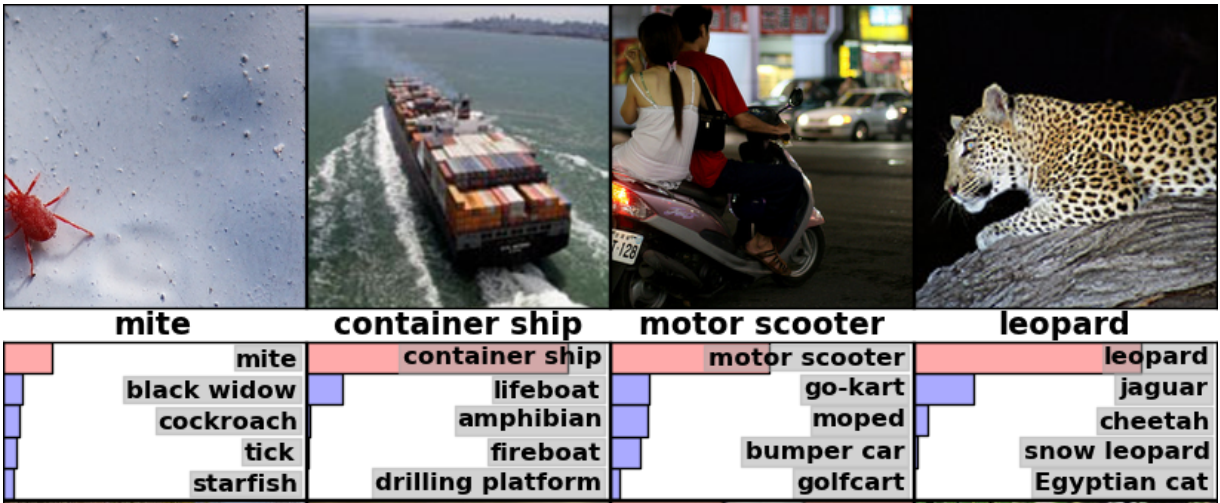
\includegraphics{AlexClassification.png}
\end{figure}
\end{center}
为了对比模型,我们检查迷行预测正确结果为"top-5 error rate",AlexNet2012年的验证数据及上得到top-5 error rate 15.3\%,Inception(GoogleLeNet)得到6.67\%,BN-Inception-v2得到4.9\%,Inception-v3得到3.46\%。
\begin{quote}
\emph{人类在ImageNet中做的怎么样,由 Andrej Karpathy 的\href{http://karpathy.github.io/2014/09/02/what-i-learned-from-competing-against-a-convnet-on-imagenet/}{博客}尝试测量人们的性能,他得到了5.1\%的top-5 error rate}
\end{quote}
下面的导航将教你如何使用Inception-v3.你将学习用Python或者C++学习分类图像成1000类,我们也将讨论如何从模型提取高级特征重用到其它的视觉任务。
\subsection{用Python API}
第一次运行时classify\_image.py将从tensorflow官网下载训练好的模型,你将需要200M左右的硬盘空间。开始从github上clone\href{https://github.com/tensorflow/models}{Google模型},然后运行命令:
\begin{lstlisting}[language=Bash]
cd models/tutorials/image/imagenet
python classify_image.py
\end{lstlisting}
上面的命令将分类下面的熊猫图片。
\begin{center}
\begin{figure}[h]
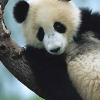
\includegraphics{cropped_panda.jpg}
\end{figure}
\end{center}
如果模型正确运行将生成下面的输出:
\begin{lstlisting}{language=Python}
giant panda, panda, panda bear, coon bear, Ailuropoda melanoleuca (score = 0.88493)
indri, indris, Indri indri, Indri brevicaudatus (score = 0.00878)
lesser panda, red panda, panda, bear cat, cat bear, Ailurus fulgens (score = 0.00317)
custard apple (score = 0.00149)
earthstar (score = 0.00127)
\end{lstlisting}
如果你希望添加其它的JPEG图片,你也许需要编辑--image\_file参数,如果你需要下载模型数据到不同的目录,你将需要指定--model\_dir到使用的目录。
\subsection{用C++ API}
你可以在生产环境上使用C++运行相同的Inception-v3模型。你可以下载包含像这样定义的GraphDef的打包文件
(从TensorFlow仓库的根目录运行)
\begin{lstlisting}[language=Bash]
curl -L "https://storage.googleapis.com/download.tensorflow.org/models/inception_v3_2016_08_28_frozen.pb.tar.gz" |
  tar -C tensorflow/examples/label_image/data -xz
\end{lstlisting}
下一步我们编译包含C++代码载入的二进制运行图,如果你已经按照\href{https://www.tensorflow.org/install/install_sources}{the instructions to download the source installation of TensorFlow}
配置了你的平台,你将能在shell终端通过下面的命令构建例子运行:
\begin{lstlisting}[language=Bash]
bazel build tensorflow/examples/label_image/...
\end{lstlisting}
你可以像这样创建一个二进制的执行文件:
\begin{lstlisting}[language=Bash]
bazel-bin/tensorflow/examples/label_image/label_image
\end{lstlisting}
用框架默认的例子图片,输出下面的结果:
\begin{lstlisting}[language=Bash]
I tensorflow/examples/label_image/main.cc:206] military uniform (653): 0.834306
I tensorflow/examples/label_image/main.cc:206] mortarboard (668): 0.0218692
I tensorflow/examples/label_image/main.cc:206] academic gown (401): 0.0103579
I tensorflow/examples/label_image/main.cc:206] pickelhaube (716): 0.00800814
I tensorflow/examples/label_image/main.cc:206] bulletproof vest (466): 0.00535088
\end{lstlisting}
在这个例子中你用一张默认的图片\href{https://en.wikipedia.org/wiki/Grace_Hopper}{Admiral Grace Hopper},你可以看到网络正确识别她的军官制服,得分0.8。
\begin{center}
\begin{figure}[H]
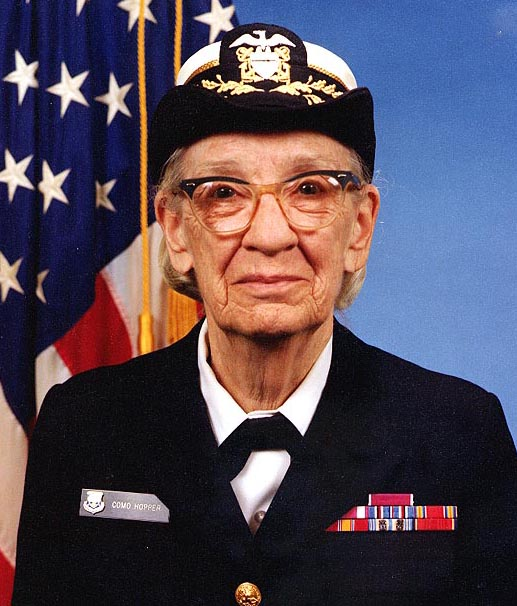
\includegraphics{grace_hopper.jpg}
\end{figure}
\end{center}
下一步提供--image=参数分辨你的图片
\begin{lstlisting}[language=Bash]
bazel-bin/tensorflow/examples/label_image/label_image --image=my_image.png
\end{lstlisting}
如果你查看\href{https://github.com/tensorflow/tensorflow/blob/master/tensorflow/examples/label_image/main.cc}{tensorflow/examples/label\_image/main.cc}你可以明白它是如何工作的,我们希望代码能帮你整合TensorFlow到你的应用,因此我们将一步步的浏览主函数。命令行参数控制文件从哪里载入,即输入图像的内容。模型希望得到$299\times299$的RGB图像,分别是input\_width,input\_height,我们需要缩放图像的像素从0-255到图能操作的一个浮点值。我们通过input\_mean和input\_std控制缩放:我们首先用像素值减去input\_mean然后除以input\_std,这些值看起来可能有点琢磨不透,但是他们被原始作者定义,她/他想训练的时候什么值被匹配,你可以看看我们如何在\href{https://github.com/tensorflow/tensorflow/blob/master/tensorflow/examples/label_image/main.cc#L88}{ReadTensorFromImageFile()}函数中如何应用一张图像。
\begin{lstlisting}[language=C++]
// Given an image file name, read in the data, try to decode it as an image,
// resize it to the requested size, and then scale the values as desired.
Status ReadTensorFromImageFile(string file_name, const int input_height,
                               const int input_width, const float input_mean,
                               const float input_std,
                               std::vector<Tensor>* out_tensors) {
  tensorflow::GraphDefBuilder b;
\end{lstlisting}
我们开始撞见亿个GraphDefBuilder对象指定一个运行或者载入的模型。
\begin{lstlisting}[language=C++]
  string input_name = "file_reader";
  string output_name = "normalized";
  tensorflow::Node* file_reader =
      tensorflow::ops::ReadFile(tensorflow::ops::Const(file_name, b.opts()),
                                b.opts().WithName(input_name));
\end{lstlisting}
然后我们开始为我们想要运行或者载入的小模型创建节点,变换大小,缩放像素值得到主函数希望得到的结果,我们创建的第一个节点是保持图像名字的tensor想要载入Const操作然后作为第一个输入传入ReadFile操作,你也许注意到我们传递b.opts()操作给所有的创建操作,参数确保节点被添加到GraphDefBuilder的模型定义。这给了一个名字给节点,
对于给一个名字节点不是严格需要的因为如果你不指定这个将自动命名,但是它使得调试变得简单
\begin{lstlisting}[language=C++]
  // Now try to figure out what kind of file it is and decode it.
  const int wanted_channels = 3;
  tensorflow::Node* image_reader;
  if (tensorflow::StringPiece(file_name).ends_with(".png")) {
    image_reader = tensorflow::ops::DecodePng(
        file_reader,
        b.opts().WithAttr("channels", wanted_channels).WithName("png_reader"));
  } else {
    // Assume if it's not a PNG then it must be a JPEG.
    image_reader = tensorflow::ops::DecodeJpeg(
        file_reader,
        b.opts().WithAttr("channels", wanted_channels).WithName("jpeg_reader"));
  }
  // Now cast the image data to float so we can do normal math on it.
  tensorflow::Node* float_caster = tensorflow::ops::Cast(
      image_reader, tensorflow::DT_FLOAT, b.opts().WithName("float_caster"));
  // The convention for image ops in TensorFlow is that all images are expected
  // to be in batches, so that they're four-dimensional arrays with indices of
  // [batch, height, width, channel]. Because we only have a single image, we
  // have to add a batch dimension of 1 to the start with ExpandDims().
  tensorflow::Node* dims_expander = tensorflow::ops::ExpandDims(
      float_caster, tensorflow::ops::Const(0, b.opts()), b.opts());
  // Bilinearly resize the image to fit the required dimensions.
  tensorflow::Node* resized = tensorflow::ops::ResizeBilinear(
      dims_expander, tensorflow::ops::Const({input_height, input_width},
                                            b.opts().WithName("size")),
      b.opts());
  // Subtract the mean and divide by the scale.
  tensorflow::ops::Div(
      tensorflow::ops::Sub(
          resized, tensorflow::ops::Const({input_mean}, b.opts()), b.opts()),
      tensorflow::ops::Const({input_std}, b.opts()),
      b.opts().WithName(output_name));
\end{lstlisting}
我们然后添加更多的节点解码文件数据为图片,转化整数为浮点值,变形然后最后运行减去和除法操作:
\begin{lstlisting}[language=C++]
  // This runs the GraphDef network definition that we've just constructed, and
  // returns the results in the output tensor.
  tensorflow::GraphDef graph;
  TF_RETURN_IF_ERROR(b.ToGraphDef(&graph));
\end{lstlisting}
在这最后我们有一个存储在变量b中的模型定义我们用ToGraphDef()转化完整的图定义
\begin{lstlisting}[language=C++]
  std::unique_ptr<tensorflow::Session> session(
      tensorflow::NewSession(tensorflow::SessionOptions()));
  TF_RETURN_IF_ERROR(session->Create(graph));
  TF_RETURN_IF_ERROR(session->Run({}, {output_name}, {}, out_tensors));
  return Status::OK();
\end{lstlisting}
我们创建一个运行图的接口tf.Session对象,运行它,指定我们想从那个节点获得输出和放输出数据到哪里,这给我们一个Tensor对象的向量,这个对象将变成一个三个对量,你可以将Tensor认为是多维数组,它保存299像素宽,299像素高。3通道的图像作为浮点值,如果你有自己的图像处理框架,你应该能用它替代,只要你在输入图像到主图中时应用相同的转换。这是用C++创建一个简单的TensorFlow图的例子,但是对于预先训练好的Inception模型我们想从文件载入一个大的定义,你可以在LoadGraph()函数中查看我们如何做的:
\begin{lstlisting}[language=C++]
// Reads a model graph definition from disk, and creates a session object you
// can use to run it.
Status LoadGraph(string graph_file_name,
                 std::unique_ptr<tensorflow::Session>* session) {
  tensorflow::GraphDef graph_def;
  Status load_graph_status =
      ReadBinaryProto(tensorflow::Env::Default(), graph_file_name, &graph_def);
  if (!load_graph_status.ok()) {
    return tensorflow::errors::NotFound("Failed to load compute graph at '",
                                        graph_file_name, "'");
  }
\end{lstlisting}
如果你已经查看的图像载入代码,一些名词应该很熟悉。想必须用一个GraphDefBuffer残生一个GraphDef对象,我们载入一个包含GraphDef的protobuf文件。
\begin{lstlisting}[language=C++]
  session->reset(tensorflow::NewSession(tensorflow::SessionOptions()));
  Status session_create_status = (*session)->Create(graph_def);
  if (!session_create_status.ok()) {
    return session_create_status;
  }
  return Status::OK();
}
\end{lstlisting}
我们从GraphDef创建一个Session对象传递它给调用器以至于我们稍后能使用。GetTopLabels()函数有些像函数载入,但是我们希望运行主图得到结果,存储它进一个按照标签最高评分的结果,像图片载入,它创建一个的GraphDefBuilder,添加一对节点上去然后运行短图割刀一对输出tensor,在这个例子中他们代表排序的分数和最好可能性的结果的索引位置。
\begin{lstlisting}[language=C++]
// Analyzes the output of the Inception graph to retrieve the highest scores and
// their positions in the tensor, which correspond to categories.
Status GetTopLabels(const std::vector<Tensor>& outputs, int how_many_labels,
                    Tensor* indices, Tensor* scores) {
  tensorflow::GraphDefBuilder b;
  string output_name = "top_k";
  tensorflow::ops::TopK(tensorflow::ops::Const(outputs[0], b.opts()),
                        how_many_labels, b.opts().WithName(output_name));
  // This runs the GraphDef network definition that we've just constructed, and
  // returns the results in the output tensors.
  tensorflow::GraphDef graph;
  TF_RETURN_IF_ERROR(b.ToGraphDef(&graph));
  std::unique_ptr<tensorflow::Session> session(
      tensorflow::NewSession(tensorflow::SessionOptions()));
  TF_RETURN_IF_ERROR(session->Create(graph));
  // The TopK node returns two outputs, the scores and their original indices,
  // so we have to append :0 and :1 to specify them both.
  std::vector<Tensor> out_tensors;
  TF_RETURN_IF_ERROR(session->Run({}, {output_name + ":0", output_name + ":1"},
                                  {}, &out_tensors));
  *scores = out_tensors[0];
  *indices = out_tensors[1];
  return Status::OK();
\end{lstlisting}
PrintTopLabels()函数得到排序接轨哦用一种友好的方式打印他们。CkeckTopLabel()函数是非常累是,但是仅仅确保顶部的标签是我们想要的,用于调试。
在最后main()结合所有的函数调用
\begin{lstlisting}[language=C++]
int main(int argc, char* argv[]) {
  // We need to call this to set up global state for TensorFlow.
  tensorflow::port::InitMain(argv[0], &argc, &argv);
  Status s = tensorflow::ParseCommandLineFlags(&argc, argv);
  if (!s.ok()) {
    LOG(ERROR) << "Error parsing command line flags: " << s.ToString();
    return -1;
  }

  // First we load and initialize the model.
  std::unique_ptr<tensorflow::Session> session;
  string graph_path = tensorflow::io::JoinPath(FLAGS_root_dir, FLAGS_graph);
  Status load_graph_status = LoadGraph(graph_path, &session);
  if (!load_graph_status.ok()) {
    LOG(ERROR) << load_graph_status;
    return -1;
  }
\end{lstlisting}
我们载入主图:
\begin{lstlisting}[language=C++]
 // Get the image from disk as a float array of numbers, resized and normalized
  // to the specifications the main graph expects.
  std::vector<Tensor> resized_tensors;
  string image_path = tensorflow::io::JoinPath(FLAGS_root_dir, FLAGS_image);
  Status read_tensor_status = ReadTensorFromImageFile(
      image_path, FLAGS_input_height, FLAGS_input_width, FLAGS_input_mean,
      FLAGS_input_std, &resized_tensors);
  if (!read_tensor_status.ok()) {
    LOG(ERROR) << read_tensor_status;
    return -1;
  }
  const Tensor& resized_tensor = resized_tensors[0];
\end{lstlisting}
载入,变形,处理输入图像
\begin{lstlisting}[language=C++]
  // Actually run the image through the model.
  std::vector<Tensor> outputs;
  Status run_status = session->Run({ {FLAGS_input_layer, resized_tensor}},
                                   {FLAGS_output_layer}, {}, &outputs);
  if (!run_status.ok()) {
    LOG(ERROR) << "Running model failed: " << run_status;
    return -1;
  }
\end{lstlisting}
我们用图像作为输入运行载入的图:
\begin{lstlisting}[language=C++]
  // This is for automated testing to make sure we get the expected result with
  // the default settings. We know that label 866 (military uniform) should be
  // the top label for the Admiral Hopper image.
  if (FLAGS_self_test) {
    bool expected_matches;
    Status check_status = CheckTopLabel(outputs, 866, &expected_matches);
    if (!check_status.ok()) {
      LOG(ERROR) << "Running check failed: " << check_status;
      return -1;
    }
    if (!expected_matches) {
      LOG(ERROR) << "Self-test failed!";
      return -1;
    }
  }
\end{lstlisting}
出于测试的目的我们可以检查确保我们得到我们想要的结果:
\begin{lstlisting}[language=C++]
// Do something interesting with the results we've generated.
  Status print_status = PrintTopLabels(outputs, FLAGS_labels);
\end{lstlisting}
最后我们打印我们输出的标签:
\begin{lstlisting}[language=C++]
 if (!print_status.ok()) {
    LOG(ERROR) << "Running print failed: " << print_status;
    return -1;
  }
\end{lstlisting}
我们用TensorFLow的State对象处理错误,它很方便因为它用ok()作为检查器检查是否出现的任何错误,然后打印出可读的错误消息,在这个例子中我们一站式对象识别,但是你应该能用类似的代码在你发现的其他模型上或者自己训练在不同的领域。我们希望这个小的例子给你一些灵感如何用TensorFlow和你的产品。
\begin{quote}
转换学习是想法,如果你知道如何很好的解决问题,你应该能转换一些解决相关问题的理解,一种执行转换学习的方法是移除网络最后的分类层提取\href{http://arxiv.org/abs/1310.1531}{next-to-last layer of the CNN},在这个例子中2048维向量,有一个关于这个如何做到的向导\href{https://www.tensorflow.org/tutorials/image_retraining}{in the how-to section}
\end{quote}
\subsection{更多学习资源}
为了学习神经网络,Michael Nielsen的\href{http://neuralnetworksanddeeplearning.com/chap1.html}{free online book},类似对于卷积神经网络Chris Olah有一些\href{http://colah.github.io/posts/2014-07-Conv-Nets-Modular/}{nice blog posts},Michael Nielsen的书有一个关于它的\href{http://neuralnetworksanddeeplearning.com/chap6.html}{greatchapter covering them}为了找出更多的卷积神经网络的实现你可以调到\href{https://www.tensorflow.org/tutorials/deep_cnn}{ deep convolutional networks tutorial},最后如果你想加速在这一领域的研究,你可以读导航中列出的最近的相关工作的论文。
\section{TensorFlow实现大规模线性模型}
tf.estimator API 提供了一些丰富的工具在TensorFlow中处理线性模型,这个章节提供了一个官员这些工具的概览,解释如下:
\begin{itemize}
  \item 线性模型是什么
  \item 为什么你想用线性模型
  \item tf.estimator如何使得在TensorFlow中建立一个线性模型变得简单
  \item 如何结合线性模型和深度学习的有点
\end{itemize}
读这个概览决定了是否tf.estimator对于你来说有用,然后做一下\href{Models tutorial}{https://www.tensorflow.org/tutorials/wide}这个概览的代码来自于这个章节,但是导航更详细的调通代码。为了明白为了理解这个概念熟悉一些基本的机器学习概念和tf.estimator是有帮助的。
\subsection{什么是线性模型}
一个线性模型用一个特征权重和作出预测,例如,如果你有关于年龄。教育年数,每周工作小时数的数据,你可以的你可以你可以了解这些权重以至于他们的权重求和评估一个人的薪水。你可以用线性模型分类,一些线性模型转化权重为一个更方便的形式,例如逻辑回归转化权重和维逻辑函数输出0-1之间的数值。但是你依然有对于每个输入特征你依然有一个权重。
\subsection{为什么你想用线性模型?}
当最近的研究已经展示了有很多层的复杂神经网络的能力为什么我们想用一个简单的模型?\newline
线性模型:
\begin{itemize}
  \item 比深度神经网络训练快速
  \item 在大型数据及上也能工作的很好
  \item 训练的时候不要求微小的学习率
  \item 相比神经网络能更简单轻松地调试,你可以检查付给给个特征的权重找出那个对于预测结果的影响最大。
  \item 对于了解机器学习提供了很好的起点
  \item 工业上广泛的使用
\end{itemize}
\subsection{tf.estimator将如何构建线性模型}
你可以通过TensorFlow建立线性模型不需要特殊的API,但是tf.estimator提供了一些工具帮助你更轻松地构建搞笑的大规模线性模型。
\subsubsection{特征列和线性模型}
设计的线性模型的大部分工作是转化原始数据为合适的输入特征,TensorFlow用FeatureColumn概念启动这些转换,一个FeatureColumn代表你的数据的单个特征,一个FeatureColumn也许代表一些像"height"或者也许代表一个像"eye\_color"的种类这里的值是来自离散的可能性像{'blue', 'brown', 'green'}。连续的特征像'height'和绝对的特征'eye\_color',在输入模型前一个单个的值可能被转化为数值序列。FeatureColumn概念让你用但一个语义单元操作特征,你可以转化选择特征来包含没有用指定索引处理的处理。
\subsubsection{稀疏列}
绝对的特征在线性模型中被转化为稀疏向量,在向量中每个可能值有一个相关的索引或者id,例如如果仅仅有三个可能的颜色代表'eye\_color'作为长度为3的向量,'brown'将变为[1,0,0],'blue'将变成[0,1,0],'green'将变成[0,0,1],这里向量被称为稀疏因为当可能值很大的时候。它们可能很长但是有很多0。尽管我们不需要用绝对列用tf.estimator线性模型,一个有力的线性模型能处理大型的稀疏向量,tf,estimator线性模型工具的稀疏特征也正是一个主要的用途。
\subsubsection{编码稀疏列}
FeatureColumn用下面的代码自动处理传统的绝对的值称为向量:
\begin{lstlisting}[language=Python]
eye_color = tf.feature_column.categorical_column_with_vocabulary_list(
    "eye_color", vocabulary_list=["blue", "brown", "green"])
\end{lstlisting}
这里的eye\_color是你的源数据的列的名字,入股你不知道所有的可能值你可以为你的绝对特征以生成FeatureColumn。对于这种情况,你将用categorical\_column\_with\_hash\_bucket(),用一盒散列函数赋值索引给特征值。
\begin{lstlisting}[language=Python]
education = tf.feature_column.categorical_column_with_hash_bucket(
    "education", hash_bucket_size=1000)
\end{lstlisting}
\subsection{特征交叉}
因为线性模型赋值独立的权重给分开的特征,他们不嫩改写东西相对重要的指定特征值的结合。如果你有一个特征'favorite\_sport'和特征'home\_city'然后你想尝试预测一个是是否喜欢船红色的衣服,你的线性模型将不能从喜欢穿红色衣服的圣路易斯的棒球粉丝中学习。你可以通过创建一个新的特征'favorite\_sport\_x\_home\_city'得到这个限制。这些特征的值对一个人仅仅链接两个源特征'baseball\_x\_stlouis',例如这个结合的特征被称为特征交叉,crossed\_column()方法使得建立特征交叉很容易
\begin{lstlisting}[language=Python]
sport_x_city = tf.feature_column.crossed_column(
    ["sport", "city"], hash_bucket_size=int(1e4))
\end{lstlisting}
连续的列,你可以像这样指定一个连续的特征:
\begin{lstlisting}[language=Python]
age = tf.feature_column.numeric_column("age")
\end{lstlisting}
尽管作为一个简单的实数,连续特征经常能直接输入给模型,TensorFlow对于排序这列提供了有用的转化。
\subsection{Bucketization}
Bucketization转化一个连续的列为绝对列。这个转换让你在交叉特征中用连续的特征,或者了解那里指定值的范围特别重要,Bucketization分隔可能值的范围为字范围称为buckets。
\begin{lstlisting}[language=Python]
age_buckets = tf.feature_column.bucketized_column(
    age, boundaries=[18, 25, 30, 35, 40, 45, 50, 55, 60, 65])
\end{lstlisting}
bucket掉入那个区域变成这个值的绝对标签。

\subsubsection{输入函数}
FeatureColumn为你的模型提供了一个指定的输入数据。标志着着如何代表和转化数据。但是他们本身不提供数据,你通过输入函数提供数据,输入函数必须返回一个tensor字典,每个键是FeatureColumn的名字。每个键的值是一个对于所有数据实例是包含特征值的tensor。查看\href{https://www.tensorflow.org/get_started/input_fn}{ Building Input Functions with tf.estimator}获取更多的关于输入函数的见解,在\href{https://www.github.com/tensorflow/tensorflow/blob/r1.3/tensorflow/examples/learn/wide_n_deep_tutorial.py}{ linear models tutorial code}中的input\_fn是实现输入函数的一个例子。在输入函数被传递给train()和evaluate()调用初始训练和测试正如下一章描述的。
\subsubsection{线性estimator}
TensorFlow的estimator给训练和分类模型提供了一个独一无二的训练评估工具。他们考虑详细的训练和评估训练允许用户集中注意力在模型输入和架构上。

为了建立一个线性estimator,你可以用tf.estimator.LinearClassfier estimator或者tf.estimator.LinearRegressor estimator分别建立分类和回归模型。

创建tensorflow estimator和运行estimator:
\begin{itemize}
  \item estimator实例,对于两个线性estimator类,你传递一个FeatureColumn列表给构造器。
  \item 调用estimator的train()方法训练它
  \item 调用estimator的evaluate()方法看看它如何工作
\end{itemize}
例如:
\begin{lstlisting}[language=Python]
e = tf.estimator.LinearClassifier(
    feature_columns=[
        native_country, education, occupation, workclass, marital_status,
        race, age_buckets, education_x_occupation,
        age_buckets_x_race_x_occupation],
    model_dir=YOUR_MODEL_DIRECTORY)
e.train(input_fn=input_fn_train, steps=200)
# Evaluate for one step (one pass through the test data).
results = e.evaluate(input_fn=input_fn_test)

# Print the stats for the evaluation.
for key in sorted(results):
    print("%s: %s" % (key, results[key]))
\end{lstlisting}
\subsection{广泛深入的学习}
tf.estimator API提供一个estimator类让你结合训练一个模型和深度神经网络。这个出色的方法结合线性模型的能力存储神经网络泛化的能力关键特征。用tf.estimator.DNNLinearCombineClassfier创建一个广而深的模型:
\begin{lstlisting}[language=Python]
e = tf.estimator.DNNLinearCombinedClassifier(
    model_dir=YOUR_MODEL_DIR,
    linear_feature_columns=wide_columns,
    dnn_feature_columns=deep_columns,
    dnn_hidden_units=[100, 50])
\end{lstlisting}
更多信息请查看\href{https://www.tensorflow.org/tutorials/wide_and_deep}{Wide and Deep Learning tutorial}。